\documentclass[12pt,a4paper]{report}

% =========================
% PAGE & COLORS
% =========================
\usepackage{geometry}
\geometry{top=2.5cm,bottom=2.5cm,left=2.5cm,right=2.5cm}

\usepackage{xcolor}
\definecolor{strengthblue}{RGB}{0,102,153}
\definecolor{weakred}{RGB}{180,40,40}
\definecolor{algeriablue}{RGB}{0,114,198}
\definecolor{lightblue}{RGB}{225,238,252}

% =========================
% FONT SYSTEM (IMPORTANT FIX)
% =========================
\usepackage{fontspec}
\usepackage{unicode-math}

\setmainfont{TeX Gyre Termes}
\setmathfont{TeX Gyre Termes Math}

% Arabic font (ONLY ONCE → FIXED)
\newfontfamily\arabicfont[Script=Arabic,Scale=1.2]{Amiri}

% =========================
% MULTILINGUAL (FIXED)
% =========================
\usepackage{polyglossia}
\setmainlanguage{english}
\setotherlanguage{arabic}

% =========================
% LISTS & STYLE
% =========================
\usepackage{enumitem}
\usepackage{wrapfig}
\usepackage{setspace}
\setstretch{1.2}

\newcommand{\good}{\textcolor{strengthblue}{\small $\blacktriangleright$}}
\newcommand{\bad}{\textcolor{weakred}{\Large $\bullet$}}

% =========================
% TABLES & GRAPHICS
% =========================
\usepackage{graphicx}
\usepackage{float}
\usepackage{booktabs}
\usepackage{array}
\usepackage{colortbl}
\usepackage{longtable}
\usepackage{multirow}
\usepackage{caption}
\usepackage{adjustbox}
\usepackage{subcaption}

% =========================
% DRAWING
% =========================
\usepackage{tikz}

% =========================
% HEADER / FOOTER
% =========================
\usepackage{fancyhdr}
\pagestyle{fancy}
\fancyhf{}
\fancyhead[L]{\leftmark}
\fancyfoot[C]{\thepage}
\renewcommand{\headrulewidth}{0.4pt}
\setlength{\headheight}{14.5pt}

% =========================
% LINKS
% =========================
\usepackage{url}
\usepackage[
    colorlinks=true,
    citecolor=blue,
    linkcolor=blue,
    urlcolor=blue
]{hyperref}

% =========================
% DOCUMENT START
% =========================
\begin{document}

\begin{titlepage}

% ===== CADRE EXTERIEUR =====
\begin{tikzpicture}[remember picture, overlay]
    \draw[black, line width=2pt] 
        ([xshift=0.8cm, yshift=-0.8cm]current page.north west) 
        rectangle 
        ([xshift=-0.8cm, yshift=0.8cm]current page.south east);
    \draw[black, line width=0.5pt] 
        ([xshift=1cm, yshift=-1cm]current page.north west) 
        rectangle 
        ([xshift=-1cm, yshift=1cm]current page.south east);
\end{tikzpicture}

% ===== EN-TETE =====
\begin{center}
    \textbf{people's Democratic Republic of Algeria} \\[6pt]
    \textbf{Ministry of Higher Education and Scientific Research} \\[6pt]
    \textbf{M'Hamed Bougara University - Boumerdes} \\[6pt]
    \textbf{Faculty of Sciences} \\[10pt]
    
\includegraphics[width=3cm]{figures/_first_page/logo1.jpg} \\[10pt]
    \textbf{Department of Computer Science}
\end{center}

\vspace{0.8cm}

% ===== FINAL YEAR PROJECT + DOMAIN =====
\begin{minipage}[t]{0.48\textwidth}
    \textbf{Final Year Project for the Award of Bachelor's Degree}
\end{minipage}
\hfill
\begin{minipage}[t]{0.48\textwidth}
    \textbf{\underline{Domain:}} Mathematics and Computer Science \\[6pt]
    \textbf{\underline{Field:}} Computer Science \\[6pt]
    \textbf{\underline{Specialty:}} Information Systems
\end{minipage}

% ===== TITRE =====
\begin{center}
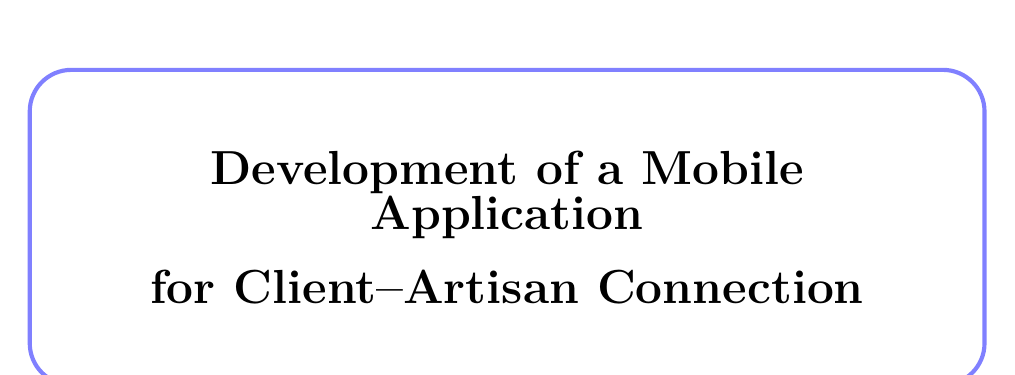
\begin{tikzpicture}
    \draw[blue!50, line width=1.5pt, rounded corners=15pt] 
        (0,0) rectangle (\textwidth, 4cm);
    \node at (0.5\textwidth, 2cm) {
        \begin{minipage}{0.9\textwidth}
            \centering
            {\LARGE \textbf{Development of a Mobile Application}} \\[10pt]
            {\LARGE \textbf{for Client--Artisan Connection}}
        \end{minipage}
    };
\end{tikzpicture}
\end{center}

\vspace{1.5cm}

% ===== PRESENTED BY ET SUPERVISOR =====
\begin{minipage}[t]{0.45\textwidth}
    \textbf{\underline{Presented by:}} \\[10pt]
    \textbf{Ms. Ikram Taftist} \\[8pt]
    \textbf{Ms. Meriem Chennouf} \\[8pt]
    \textbf{Ms. Nour El Houda Akhdari} \\[8pt]
    \textbf{Ms. Sofia Oubaziz}
\end{minipage}
\hfill
\begin{minipage}[t]{0.45\textwidth}
    \textbf{\underline{Supervisor:}} \\[8pt]
    \textbf{Ms. Samiya Hamadouche} \\[12pt]
    \textbf{\underline{Examiner :}} \\[8pt]
    \textbf{Mr. Nouasri Amine} \\[12pt]
    \textbf{\underline{Defended on}} : \\[6pt]
    26/05/2026
\end{minipage}

\vspace{\fill}

% ===== ANNEE ACADEMIQUE =====
\begin{center}
    \textbf{Academic Year: 2025/2026}
\end{center}

\end{titlepage}

\clearpage
\thispagestyle{empty}
\null
\newpage

\pagenumbering{roman}
% ===== DEDICATION 1 - Meriem =====
\newpage
\thispagestyle{fancy}
\begin{center}
    {\Large \textbf{Dedication}}
\end{center}

\vspace{0.5cm}

\begin{center}
    \textit{بسم الله الرحمن الرحيم}
\end{center}

\vspace{0.5cm}

Tout d'abord, je tiens à remercier Dieu de m'avoir donné la force et le courage d'accomplir ce modeste travail.

\vspace{0.5cm}

Je dédie ce travail :

\vspace{0.3cm}

\textbf{À la petite fille que j'étais autrefois}

Tu es aimée, tu es entendue, tu es vue. Je suis devenue ce refuge sûr que tu espérais, cette force tranquille que tu cherchais dans les tempêtes. Aujourd'hui, je te rends hommage avec tendresse et fierté, car je suis fière de la femme que je suis devenue, fière du chemin parcouru, des peurs affrontées et des rêves réalisés. Et surtout, je suis enfin heureuse.

\begin{center}
    \textit{Ce projet est pour toi}
\end{center}

\vspace{0.3cm}

\textbf{À ma très chère mère}

Ce pilier de ma vie, cette femme au cœur immense dont l'amour inconditionnel et les prières silencieuses m'ont porté dans les moments les plus difficiles. Aucune dédicace, aucun mot, aucune phrase ne pourrait exprimer l'amour, la reconnaissance et le respect que j'ai pour toi. Tu es et tu resteras ma plus belle lumière.

\vspace{0.3cm}

\textbf{À mon cher père}

Cet homme de dignité et de sagesse, qui s'est sacrifié sans compter pour que je puisse atteindre mes rêves. Tu m'as appris que la persévérance est la clé de tout succès. Ta fierté est ma plus belle récompense et ton soutien mon plus grand trésor.

\vspace{0.3cm}

\textbf{À ma chère sœur Bouchra}

Ma confidente, ma douceur et ma complice de toujours. Merci pour ta présence, ton soutien sincère et ton amour fraternel qui m'ont accompagné tout au long de ce chemin.

\vspace{0.3cm}

\textbf{À mon cher frère Azzedine}

Mon ami, mon pilier et mon confident. Merci pour chaque mot d'encouragement, chaque geste de soutien et chaque moment partagé qui ont rendu ce voyage plus léger.

\vspace{0.3cm}

\textbf{À mes chers amis}

Vous qui avez partagé avec moi les rires et les larmes, les doutes et les victoires. Votre amitié sincère a été un véritable cadeau sur ce parcours. Merci d'avoir toujours cru en moi.


\newpage
\thispagestyle{fancy}

\begin{center}
    {\Large \textbf{Dedication}}
\end{center}

\vspace{0.5cm}

\begin{center}
    {\Large \textbf{بِسْمِ اللهِ الرَّحْمٰنِ الرَّحِيم}}
\end{center}

\vspace{0.5cm}

{\arabicfont
\begin{RTL}

الحمدُ لله الذي بنعمته تتمّ الصالحات، أحمده سبحانه حمدًا كثيرًا طيبًا مباركًا فيه، فقد منَّ عليَّ بإتمام مشوارٍ جامعيٍّ جديد تُوِّج بنيل شهادة الليسانس، فله الحمد أولًا وآخرًا على ما وفّق ويسّر. وأسأله عزّ وجلّ أن يرزقني علمًا نافعًا أُفيد به غيري، وأن يجعل ما تعلمناه وعملنا به في ميزان حسناتنا.

\vspace{0.4cm}

أتقدّم بخالص الشكر والامتنان إلى كلّ من كان سندًا لي وداعمًا خلال هذه السنوات الثلاث، وعلى رأسهم والداي العزيزان، اللذان كانا نعم العون والسند.

\vspace{0.3cm}

\textbf{شكراً أبي، شكراً أمي،} على كلّ ما بذلتماه من تعبٍ وصبرٍ ودعاء، وعلى دعمكما المتواصل الذي كان يدفعني للاستمرار وتجاوز كلّ الصعوبات، فجزاكما الله عنّي خير الجزاء وبارك في عمركما.

\vspace{0.4cm}

كما أتوجّه بالشكر إلى إخوتي وأختي الأعزاء، الذين كانوا مصدرًا للطمأنينة والابتسامة رغم التعب والمشقة، وإلى أخي الصغير الذي كان خير أنيسٍ ورفيقٍ لي في طريق العودة، دون كللٍ أو تذمّر، أسأل الله أن يرزقه من واسع فضله ويوفّقه لما يحب ويرضى.

\vspace{0.4cm}

ولا يفوتني أن أتقدّم بجزيل الشكر إلى أساتذتي الكرام، وكلّ من علّمني حرفًا أو قدّم لي علمًا أو نصيحة. كما أخصّ بالشكر الأساتذة المتفهّمين أصحاب الأخلاق الرفيعة، الذين جعلوا من طلب العلم متعةً وشغفًا لا ينطفئ.

\vspace{0.4cm}

وأشكر صديقاتي ورفيقات دربي، اللواتي كنّ خير سندٍ ورفقة طوال سنوات الدراسة، فقد خفّفن عنّي ضغوط الأيام الصعبة، وشاركني لحظات التعب والنجاح، فكانت الجامعة أجمل بوجودهن. أسأل الله أن يحفظكن ويوفّقكن في مستقبلكن العلمي والمهني.

\vspace{0.4cm}

وفي الختام، نحمد الله حمدًا كثيرًا على إتمام هذا المشروع الذي قدّمناه أنا وزميلاتي بكلّ إخلاصٍ واجتهاد، ووضعنا فيه جزءًا من جهدنا ووقتنا وطموحنا. نسأل اللهم أن تجعله علمًا نافعًا وسببًا للخير والمنفعة، وأن تبارك لنا فيما تعلمنا، وتزيدنا علمًا وتوفيقًا، إنّك وليّ ذلك والقادر عليه.

\end{RTL}
}
% ===== DEDICATION 2 - Sofia =====
\newpage
\thispagestyle{fancy}
\begin{center}
    {\Large \textbf{Dedication}}
\end{center}

\vspace{0.5cm}

Je dédie ce travail de fin d'études à toutes les personnes qui ont occupé une place importante dans ma vie et qui m'ont accompagnée, de près ou de loin, durant ce long parcours rempli d'efforts, de doutes, de sacrifices et d'espoir.

\vspace{0.3cm}

\textbf{À ma famille}, pour votre amour inconditionnel, votre patience, vos encouragements et votre présence dans les moments les plus difficiles. Merci d'avoir toujours cru en moi même lorsque moi-même je doutais. Votre soutien a été ma plus grande force. Une pensée toute particulière à mon frère \textbf{Idir} et ma sœur \textbf{Katia}, pour votre présence, vos conseils, votre soutien moral et tous ces petits gestes qui ont compté plus que vous ne l'imaginez. Vous avez été une source de motivation et de réconfort tout au long de cette aventure. Savoir que je pouvais compter sur vous m'a aidée à avancer malgré la fatigue, le stress et les périodes compliquées.

\vspace{0.3cm}

\textbf{À mes amis(es)}, merci pour les moments de rire, les discussions, l'entraide, les encouragements et la présence sincère durant les périodes de pression. Vous avez rendu ce parcours plus léger et plus beau.

\vspace{0.3cm}

\textbf{À mon groupe de PFE}, merci pour les efforts partagés, la patience, les idées, les difficultés traversées ensemble et tous les moments vécus durant ce projet. Ce travail représente aussi une aventure humaine faite de collaboration, de persévérance et d'apprentissage.

\vspace{0.3cm}

\textbf{À mes grands-parents}, paix à leurs âmes, même si vous n'êtes plus parmi nous aujourd'hui, votre amour, vos valeurs et vos prières continuent de m'accompagner chaque jour. J'aurais aimé que vous soyez présents pour voir ce moment si important de ma vie. Cette réussite vous est dédiée avec beaucoup d'amour et d'émotion.

\vspace{0.3cm}

Et enfin… je me dédie aussi ce travail \textbf{à moi-même}. À cette version de moi qui a continué malgré le stress, les nuits difficiles, la pression, les moments de découragement et la peur de ne pas y arriver. À toutes les fois où j'ai dû être forte, persévérer et me relever seule. Le chemin n'a pas été facile, mais je suis restée debout jusqu'au bout.

\vspace{0.3cm}

Aujourd'hui, je suis fière de moi, fière du chemin parcouru, fière de ne pas avoir abandonné malgré toutes les difficultés. Ce mémoire représente bien plus qu'un projet académique : il représente une preuve de ma détermination, de ma patience et de ma capacité à avancer même dans les moments compliqués.

\vspace{0.3cm}

Que ce travail soit le début d'un avenir rempli de réussite, de bonheur et de nouvelles ambitions.
% ===== DEDICATION 3 - Nour =====
\newpage
\thispagestyle{fancy}

\begin{center}
    {\Large \textbf{Dedication}}
\end{center}

\vspace{0.5cm}

To my parents, thank you for your unwavering presence throughout my journey. I am deeply grateful for all the sacrifices you have made for me.

\vspace{0.3cm}

To my grandparents, whose home was always open to me and became the place where I spent much of my life, thank you for raising me with love, care, and guidance.

\vspace{0.3cm}

Particulièrement à ma grand-mère, qui n’a pas eu la chance de terminer ses études, mais qui a toujours profondément cru en la valeur de l’éducation et a encouragé toutes les femmes autour d’elle, y compris moi, à poursuivre leurs objectifs. J’ai choisi d’écrire cette partie en français afin qu’elle puisse la comprendre. Merci pour ta confiance constante en moi, ton soutien, ainsi que pour la force et la gentillesse qui continuent de m’inspirer.

\vspace{0.3cm}

To my grandfather on my father’s side, although we were not in close contact throughout much of my life, I still carry your memory with me and hold it close to my heart.

\vspace{0.3cm}

To my aunts, thank you for your care, encouragement, and for always making me feel supported throughout the years. You have been like older sisters to me in so many ways.

\vspace{0.3cm}

And especially to my aunt Isma, whose kindness, support, and generosity have meant more to me than words can express. Thank you for always being there for me, believing in me, and caring for me.

\vspace{0.3cm}

And to someone very special to me, thank you for your constant support, encouragement, and for being my companion throughout this journey. Your belief in me, your love, and your companionship have meant more than you know.

\vspace{0.3cm}

This work is dedicated to all of you.
\newpage
\thispagestyle{fancy}

\begin{center}
    {\Large \textbf{Dedication}}
\end{center}

\vspace{0.8cm}

\textbf{To our supervisor, Madame Hamadouche Samya}

\vspace{0.3cm}

We would like to express our sincere gratitude and sincere appreciation for your valuable guidance, patience, and continuous support throughout this project.

Your scientific rigor, insightful advice, and constant availability have been a great source of motivation and have significantly contributed to the success of this work.

Working under your supervision has been both an honor and a privilege. We are truly grateful for your trust, encouragement, and dedication.

\vspace{0.3cm}

Thank you for everything you have done for us.
\chapter*{Abstract}
\addcontentsline{toc}{chapter}{Abstract}

This project involves the design and development of a mobile application called Allo Artisan, aimed at connecting clients with artisans in Algeria. Following an analysis of existing solutions and their limitations, we proposed a solution built around three main axes: trust, functionality, and accessibility.

The application provides key features such as QR code identity verification, diploma validation, a multi-criteria search system, an availability calendar, and a post and notification mechanism for service requests.

Technically, the application was developed using Flutter for the mobile interface, Go (Golang) for the backend, and PostgreSQL as the database management system, deployed via Docker.

\textbf{Keywords:} Mobile application, client-artisan connection, Flutter, Go, PostgreSQL.

\vspace{1cm}

% =========================
% ===== Résumé (section arabe → français) =====
\section*{الملخص}
\addcontentsline{toc}{chapter}{الملخص}

{\arabicfont
\begin{RTL}


\noindent
يتناول هذا المشروع تصميم وتطوير تطبيق هاتف محمول يُدعى \textenglish{«Allo Artisan»}، يهدف إلى تسهيل عملية الربط بين الزبائن والحرفيين في الجزائر.

بعد دراسة وتحليل التطبيقات الموجودة في نفس المجال والتعرّف على حدودها ونقاط ضعفها، قمنا باقتراح حل يعتمد على ثلاثة محاور أساسية: الثقة، الوظائف، وسهولة الاستخدام.

يوفّر التطبيق مجموعة من الخصائص الأساسية، من بينها: التحقق من هوية الحرفي باستخدام \textenglish{QR}، التحقق من الشهادات والوثائق المهنية، نظام بحث متعدد المعايير، تقويم لتحديد فترات التوفر، بالإضافة إلى نظام للمنشورات والإشعارات الخاصة بطلبات الخدمات العادية والمستعجلة.

من الناحية التقنية، تم تطوير التطبيق باستخدام \textenglish{Flutter} لتطوير واجهة الهاتف المحمول، و\textenglish{Go (Golang)} لتطوير الجزء الخلفي وإنشاء واجهة \textenglish{API REST}، إضافةً إلى \textenglish{PostgreSQL} كنظام لإدارة قواعد البيانات، مع استخدام \textenglish{Docker} لضمان نشر مستقر وقابل للنقل.

\vspace{0.3cm}
\textbf{الكلمات المفتاحية:} تطبيق هاتف محمول، الربط بين الزبائن والحرفيين، Flutter، Go، PostgreSQL.

\end{RTL}
}
% Table of Contents
% ======================
\tableofcontents
\newpage
\addcontentsline{toc}{chapter}{List of Tables}
\listoftables
\newpage

\addcontentsline{toc}{chapter}{List of Figures}
\listoffigures
\newpage
\chapter*{General Introduction}
\addcontentsline{toc}{chapter}{General Introduction}
\markboth{General Introduction}{General Introduction}
\thispagestyle{fancy}
In today's rapidly evolving digital landscape, mobile applications have become essential tools 
for simplifying everyday tasks and improving access to services. Among the most pressing 
challenges faced by Algerian households is the difficulty of finding reliable, qualified, and 
available artisans for urgent needs such as plumbing repairs, electrical installations, or 
mechanical interventions. Despite the existence of numerous skilled professionals in the 
market, the lack of an efficient and trustworthy platform to connect them with potential clients 
creates a significant gap in the local service ecosystem.

A review of existing solutions such as Khedamni, De9de9, and Afriha reveals recurring 
limitations: absence of identity verification, lack of availability management, restricted search 
options, and insufficient trust mechanisms. These shortcomings motivated us to propose a 
more robust and user-centered alternative  \textbf{Allo Artisan}  a mobile application designed to 
bridge the gap between clients and artisans through a secure, transparent, and intuitive 
platform built around three core principles: \textbf{trust, functionality, and accessibility}.

This document is structured into three chapters. \newline\textbf{Chapter 1} presents a comparative analysis of 
existing applications, defines the problem statement, and describes our proposed solution 
strategy. \newline\textbf{Chapter 2} covers the complete UML modeling of the system, including use case, 
sequence, class, and activity diagrams. \newline\textbf{Chapter 3} details the implementation phase, 
presenting the tools and technologies used alongside the main interfaces of the application.

% ======================
% Chapters
% ======================
\newpage
\pagestyle{fancy}
\pagenumbering{arabic}
\setcounter{page}{1}
\chapter{Existing System Analysis}

\section{Introduction}

This chapter is dedicated to the study and analysis of \textbf{existing solutions} in the same domain as our project. Reviewing existing applications represents a \textbf{fundamental step} in the development of any new system, as it provides a clear understanding of current market solutions and their functionalities. Through this analysis, we aim to examine how these applications operate, evaluate the \textbf{services they provide to users}, and identify their \textbf{strengths} as well as their \textbf{limitations}. 

This study will enable us to determine the aspects that require improvement and to define the \textbf{requirements} necessary for designing a more \textbf{effective}, \textbf{reliable}, and \textbf{competitive application}.


\section{Review of Existing Solutions and Applications}

To better understand the current state of existing solutions, we will analyze a selection of popular applications in this domain, namely \textit{\textbf{Khedamni}}, \textit{\textbf{De9de9}}, and \textit{\textbf{Afriha}}. Each application will be examined based on its \textbf{main features},\textbf{ strengths}, and\textbf{ weaknesses} in order\textbf{ to highlight their limitations} and \textbf{identify opportunities for improvement}.
% =======================
% Khedamni
% =======================
\subsubsection{\underline{Khedamni}}
\textit{\textbf{Khedamni}} is a mobile application available on the Google Play Store, with over 10,000 downloads and a rating of 4.4 stars based on 207 reviews.

\begin{center}
    
\includegraphics[width=2.5cm]{figures/_first_page/khedmni .png} 
    \par
    \textbf{Khedamni Logo}
\end{center}

\textbf{Weaknesses:}
\begin{itemize}[label=\bad, leftmargin=1.2cm, itemsep=2pt]
\item Search limited to filtering by wilaya and commune only
\item Many professionals have limited feedback, making it hard to assess service quality
\item No diploma required during account creation, profiles lack professionalism
\item No calendar feature, so users cannot check artisan availability
\item Profiles display very little information overall
\end{itemize}

\textbf{Strengths:}
\begin{itemize}[label=\good, leftmargin=1.2cm, itemsep=2pt]
\item Clean and professional interface
\item Home page displays client posts filtered by wilaya, commune, and category
\item Account creation is simple and straightforward
\item Good use of post status indicators (e.g., ``en attente'', replies)
\end{itemize}



% =======================
% De9de9
% =======================
\subsubsection{\underline{De9de9}}
\textit{\textbf{De9de9 }}is a mobile and web application available on the Google Play Store, with over 50,000 downloads and a rating of 4.1 stars based on 120 reviews.

\begin{center}
    
\includegraphics[width=2.5cm]{figures/_first_page/d9d9.png} 
    \par
    \textbf{De9de9 Logo}
\end{center}

\textbf{Weaknesses:}
\begin{itemize}[label=\bad, leftmargin=1.2cm, itemsep=2pt]
\item No consistent standards in account creation; mix of professional and irrelevant profiles, which is unfair to skilled users
\item No verification framework to validate identities or qualifications; no diploma required
\item Guest access is very restricted, preventing visitors from building enough trust to register
\end{itemize}

\textbf{Strengths:}
\begin{itemize}[label=\good, leftmargin=1.2cm, itemsep=2pt]
\item Richly detailed artisan profiles: questionnaire, work gallery, itemized pricing, availability calendar, and ratings
\item Wide diversity of service categories with many subcategories
\end{itemize}



% =======================
% Afriha
% =======================
\subsubsection{\underline{Afriha}}
\textit{\textbf{Afriha}} is a mobile and web application available on the Google Play Store, with over 10,000 downloads and a rating of 4.0 stars based on 24 reviews.

\begin{center}
    
\includegraphics[width=2.5cm]{figures/_first_page/afriha.png} 
    \par
    \textbf{Afriha Logo}
\end{center}

\textbf{Weaknesses:}
\begin{itemize}[label=\bad, leftmargin=1.2cm, itemsep=2pt]
\item Mandatory GPS activation undermines trust and discourages new users
\item Home page displays artisan accounts in a random and unclear order
\item No diploma required, profile names appear unprofessional
\item Search filtering limited to category only, which can raise safety concerns
\item No calendar, profiles lack pricing and scheduling details
\item Post functionality is very limited
\end{itemize}

\textbf{Strengths:}
\begin{itemize}[label=\good, leftmargin=1.2cm, itemsep=2pt]
\item Search uses selection-based navigation instead of free-text input
\item Wide variety of service categories with many associated services
\end{itemize}

\section{Problem Statement}
After conducting research by reading user reviews of existing applications, we collected 
their needs. Based on this, we identify the problem that should be addressed through our proposed application : \newline
The identified shortcomings of current applications reveal a fundamental gap in addressing the needs of both end users and skilled artisans, highlighting the need for a more robust, scalable, and user-centered solution adapted to modern service ecosystems

\section{Proposed an Adopted Solution}
This section presents the main design directions of the proposed application, which are based on the analysis of existing systems and identified user needs. The proposed solution is structured around three main axes: \textbf{trust}, \textbf{functionality}, and \textbf{usability \& accessibility}, which together define the core principles of our application.

\subsubsection{\large1. \underline{Trust}}
\begin{itemize}
    \item[$\bullet$] Each artisan is assigned a \textbf{QR code} linked to their profile, allowing clients to verify their identity before receiving any service.
    
    \item[$\bullet$] Artisan registration requires a \textbf{formal verification process}, including personal information and supporting documents such as diplomas or professional licenses. Accounts are reviewed before activation.
    
    \item [$\bullet$] A \textbf{reliable review system} is implemented, where ratings can only be submitted after service confirmation from both the client and the artisan, ensuring authenticity.
    
    \item[$\bullet$] A \textbf{progressive rating system} is used to reflect the artisan’s most recent performance more accurately.
    
    \item[$\bullet$] The system includes a \textbf{Visitor Mode}, allowing users to browse the application without registration, improving accessibility and transparency.
    
    \item[$\bullet$] The application does not rely on GPS tracking; instead, users manually select their location (wilaya and commune), with an optional \textbf{distance-based search (km zone)} to find nearby artisans.
\end{itemize}

\subsubsection{\large2. \underline{Features}}
\begin{itemize}
    \item[$\bullet$] An \textbf{advanced search system} allows users to filter artisans by category and location (wilaya and commune), with an additional \textbf{distance-based filter (km zone)}.
    
    \item[$\bullet$] Artisans can switch between \textbf{Active and Inactive modes}, controlling their visibility and availability.
    
    \item[$\bullet$] A \textbf{post system} enables clients to publish requests (urgent or non-urgent), which are sent as notifications to active artisans in the same category and area. Artisans can also share their work and interact through comments and reactions.
    
    \item[$\bullet$] Each artisan profile includes a \textbf{calendar showing availability and booked days}, without exposing detailed appointment information to preserve privacy.
\end{itemize}

\subsubsection{\large3. \underline{Usability \& Accessibility}}
\begin{itemize}
    \item[$\bullet$] The platform supports \textbf{three languages (Arabic, French, English)} to serve a wide range of users.
    \item[$\bullet$] Users can \textbf{follow and save artisans} for quick and easy access later.
    \item[$\bullet$] Only \textbf{active artisans} are displayed in search results to improve efficiency.
    \item[$\bullet$] The interface is designed to be \textbf{simple, clear, and intuitive}, suitable for users of all technical levels.
\end{itemize}
\begin{figure}[H]
    \centering
    
\includegraphics[width=0.98\textwidth]{figures/_first_page/chapter_picture.jpg}
    \caption{A Service-Based Application}
    \label{fig:a service-based application}
\end{figure}
\section{Conclusion}

In this chapter, we conducted a \textbf{comprehensive study} of existing applications by analyzing their \textbf{strengths and weaknesses} from the users’ perspective. This evaluation enabled us to identify \textbf{relevant improvements} and \textbf{innovative solutions} that will be integrated into our application in order to enhance its \textbf{performance}, \textbf{usability}, and \textbf{competitiveness} in the market. 

In the next chapter, we will proceed to the implementation of the proposed solutions through the \textbf{System Modeling} phase using \textbf{UML diagrams}.



\chapter{Application Modeling}
\section{\textbf{Introduction}}
    In this chapter, we will study several UML (Unified Modeling Language) models of a system. Some models present the system from the users’ point of view, others illustrate its internal structure, while some provide a global or detailed vision of the system. These models complement each other and can be combined. They are developed throughout the entire system development life cycle, from requirements expression to the design phase,
\textbf{The application brings together five main actors}: the Visitor, the Client, the Artisan, the Moderator, and the Administrator   
\section{Requirements expression}
 \subsection{Definition of Use Case Diagram}

Use case diagram are usually referred to as behavior diagram used to describe a set of 
actions (use cases) that some system should or can perform in collaboration with one or 
more external users of the system (actors). Each use case should provide some observable 
and valuable result to the actors or other stakeholders of the system\cite{ref1}.

\subsection{Identification of the actors}

There are five actors who can use our application:

\begin{enumerate}
    \item \textbf{Visitor:} an unauthenticated person who can access limited public features of the \\ application.
    \item \textbf{Client:} a registered user who can access the full feature of the application.
    \item \textbf{Artisan:} a registered professional who offers services on the platform.
    \item \textbf{Moderator:} a system manager responsible for controlling and supervising the application.
    \item \textbf{Administrator:} a system manager responsible for adding or rejecting a moderator and to help the moderator in its tasks.
\end{enumerate}

Each actor interacts with the system according to their role and permissions, which will be 
reflected in the use case diagram.

\subsection{Identification of the use case}
In this table \ref{tab:usecase}, each actor has been defined with their own use cases:
\begin{table}[H]
\centering
\renewcommand{\arraystretch}{1.1}
\begin{tabular}{|>{\bfseries\centering\arraybackslash}m{3cm}|>{\arraybackslash}m{10cm}|}
\hline
\cellcolor[HTML]{1F4E79}\textcolor{white}{\textbf{Actor}} & \cellcolor[HTML]{1F4E79}\textcolor{white}{\textbf{Use Case}} \\
\hline
\textbf{Visitor} & View a post \\
\hline
\multirow{8}{*}{\textbf{Client}} & Create an account \\
 & Interact with an artisan's post \\
 & Search an artisan \\
 & View artisan's profile \\
 & Manage an appointment \\
 & Check the artisan profile by QR code \\
 & Rate an artisan after service \\
 & Exchange message with artisan \\
\hline
\multirow{7}{*}{\textbf{Artisan}} & Register an account \\
 & Process request \\
 & View the notification \\
 & Set the availability in a calendar \\
 & Set status \\
 & Publish a new post \\
 & Exchange message with client \\
\hline
\multirow{3}{*}{\textbf{Moderator}} & Approve post \\
 & Manage reports \\
 & Manage accounts \\
\hline
\textbf{Administrator} & Manage moderator \\
\hline
\end{tabular}
\caption{Use cases by actor}
\label{tab:usecase}
\end{table}
\subsection{presentation of Use case diagram}
The following figure \ref{fig:use-case-diagram} illustrates the use case diagram of the application:

\begin{figure}[H]
    \centering
    
\includegraphics[width=0.98\textwidth]{figures/_first_page/use case 7.drawio.png}
    \caption{Use Case Diagram}
    \label{fig:use-case-diagram}
\end{figure}
\section{Analyse}
This point describes in detail the behavior and interactions between the different components, and for this purpose, we use:
\subsection{Definition of the Sequence Diagram}
 A sequence diagram represent interactions between lifelines ,and illustrates interactions from a temporal perspective, particularly the chronological sequence of messages exchanged between lifelines\cite{ref3}
\subsection{Example of the Sequence Diagram and their Textual Descriptions}
In this part, we will present the sequence diagrams along with their textual descriptions for certain use cases of our system.
\subsubsection{Use Case :'Register an Account Artisan' }
The following figure(figure:\ref{fig:register account _ artisan})represents the sequence diagram of the <<Register an Artisan account>> use case: 
\begin{figure}[H]
    \centering
    
\includegraphics[width=0.98\textwidth]{figures/_first_page/sequance-client_request_service.drawio.png}
    \caption{sequence diagram of the <<register an artisan account>> use case}
    \label{fig:register account _ artisan}
\end{figure}
The following table (Table:\ref{tab:create-artisan}) represents the textual description corresponding to the previous sequence diagram(figure:\ref{fig:register account _ artisan}):
\begin{table}[H]
\centering
\renewcommand{\arraystretch}{1}
\begin{tabular}{|>{\bfseries\arraybackslash}m{4cm}|>{\arraybackslash}m{10cm}|}
\hline
\multicolumn{2}{|c|}{\cellcolor[HTML]{1F4E79}\textcolor{white}{\textbf{Register Artisan Account}}} \\
\hline
Title & Register Artisan Account \\
\hline
Actor & Artisan \\
\hline
Objective & Register a new artisan account in the system. \\
\hline
Precondition & The artisan must have a valid email address. \\
\hline
Nominal Scenario &
\begin{minipage}[t]{10cm}
\vspace{1pt}
    1.The Artisan submits registration details.\\
    2. The Application queries the Database to verify if the email already exists.\\
    1.1. The Database returns that the email is available.\\
    3. The Application saves the artisan data with "Pending" status.\\
    1.1. The Database confirms successful record creation.\\
    1.2. The Application notifies the Artisan that the registration has been submitted and is awaiting confirmation.
\vspace{1pt}
\end{minipage} \\
\hline
Alternative Scenario & \textbf{A1: If the email already exists.} \newline
1.1. The Application notifies the Artisan that the email is already registered. \\
\hline
\end{tabular}
\caption{Textual Description of the Use Case <<Register an Artisan Account>>}
\label{tab:create-artisan}
\end{table}

\subsubsection{Use Case :'authentication'}
The following figure (figure:\ref{fig:authentication sequence diagram}) represents the sequence diagram of the “Authentication” use case 
\begin{figure}[H]
    \centering
    
\includegraphics[width=0.98\textwidth]{figures/_first_page/sequance-auth.drawio (1).png}
    \caption{sequence diagram of `Authentication` use case}
    \label{fig:authentication sequence diagram}
\end{figure}
The following table (Table:\ref{tab:authentication}) represents the textual description corresponding to the previous sequence diagram(figure:\ref{fig:authentication sequence diagram}):
\begin{table}[H]
\centering
\renewcommand{\arraystretch}{1.1}
\begin{tabular}{|>{\bfseries\arraybackslash}m{4cm}|>{\arraybackslash}m{12cm}|}
\hline
\multicolumn{2}{|c|}{\cellcolor[HTML]{1F4E79}\textcolor{white}{\textbf{User Authentication}}} \\
\hline
Title & User Authentication \\
\hline
Actor & User (Artisan or Admin) \\
\hline
Objective & Log into the system using credentials. \\
\hline
Precondition & The user has a previously created and validated account. \\
\hline
Nominal Scenario &
\begin{minipage}[t]{12cm}
\vspace{1pt}
1. The User fills in the login form.\\
   2.The Application sends the credentials to the Database for verification.\\
    2.1.The Database returns a successful result.\\
    1.2.The Application redirects the User to the main application.
\vspace{1pt}
\end{minipage} \\
\hline
Alternative Scenario & \textbf{A1: Invalid credentials.} \newline
1.1. The Application displays an error message. \\
\hline
\end{tabular}
\caption{Textual Description of the Use Case <<Authentication>>}
\label{tab:authentication}
\end{table}
\subsubsection{Use Case :'Schedule an appointment'}
The following figure (Figure\ref{fig:request service}) represents the sequence diagram of the<<Schedule an appointment>>use case  
\begin{figure}[H]
    \centering
    
\includegraphics[width=0.98\textwidth]{figures/_first_page/sequance-create_account_artisan.drawio (1).png}
    \caption{Schedule an appointment sequence diagram}
    \label{fig:request service}
\end{figure}
 The following table (Table\ref{tab:Schedule an appointment}) represents the textual description corresponding to the previous sequence 
diagram(Figure\ref{fig:request service}):
\begin{table}[H]
\centering
\renewcommand{\arraystretch}{1}
\begin{tabular}{|>{\bfseries\arraybackslash}m{4cm}|>{\arraybackslash}m{11cm}|}
\hline
\multicolumn{2}{|c|}{\cellcolor[HTML]{1F4E79}\textcolor{white}{\textbf{Schedule an appointment}}} \\
\hline
Title & Schedule an appointment \\
\hline
Actor & Client \\
\hline
Objective & Allow a client to request a service and book an available artisan. \\
\hline
Precondition &
\begin{minipage}[t]{10cm}
\vspace{4pt}
$\bullet$ The Client is authenticated. \\
$\bullet$ There are available artisans in the system.
\vspace{4pt}
\end{minipage} \\
\hline
Nominal Scenario &
\begin{minipage}[t]{10cm}
\vspace{4pt}
1.1. The Client sends a service request. \\
1.2. The Client selects preferred date and time. \\
2.1. The Client App saves the service request details in the Database. \\
2.2. The Database returns a list of available providers. \\
2.4. The Client App notifies the Client that an artisan is available. \\
1.3. The Client reviews the interested Artisan's profile and confirms the booking.
\vspace{4pt}
\end{minipage} \\
\hline
Alternative Scenario &
\begin{minipage}[t]{10cm}
\vspace{4pt}
\textbf{A1 (High Urgency):} \\
2.3. The Client App notifies all available providers about the urgent request. \\
3.1. The system sends push notification to available Artisans. \\
3.2. The Artisan views the request details. \\
3.3. The Artisan shows interest (optional). \\
1.3. The Client reviews the interested Artisan's profile and confirms the booking.
\vspace{4pt}
\end{minipage} \\
\hline
\end{tabular}
\caption{Use case: Schedule an appointment}
\label{tab:Schedule an appointment}
\end{table}




\subsubsection{Use Case :approve artisan account creation}
The following figure (figure:\ref{fig:Approve Artisan Account Creation}) represents the sequence diagram of the <<Approve artisan account creation>> use case 
\begin{figure}[H]
  \centering
    
\includegraphics[width=0.98\textwidth]{figures/_first_page/admin_val.jpg}
    \caption{approve artisan account sequence diagram}
    \label{fig:Approve Artisan Account Creation}
\end{figure}
The following table (Table:\ref{tab:validate-artisan}) represents the textual description corresponding to the previous sequence diagram(Figure\ref{fig:Approve Artisan Account Creation}):
\begin{table}[H]
\centering
\renewcommand{\arraystretch}{1}
\begin{tabular}{|>{\bfseries\arraybackslash}m{4cm}|>{\arraybackslash}m{12cm}|}
\hline
\multicolumn{2}{|c|}{\cellcolor[HTML]{1F4E79}\textcolor{white}{\textbf{Approve Artisan Account}}} \\
\hline
Title & Approve Artisan Account \\
\hline
Actor & Admin \\
\hline
Objective & Approve a pending artisan account. \\
\hline
Precondition &
\begin{minipage}[t]{10cm}
\vspace{4pt}
\begin{itemize}[leftmargin=*, nosep]
    \item The Admin must be authenticated.
    \item There are pending artisan accounts.
\end{itemize}
\vspace{4pt}
\end{minipage} \\
\hline
Nominal Scenario &
\begin{minipage}[t]{10cm}
\vspace{4pt}
    1.The Admin views the list of pending artisans.\\
    2.The Application retrieves pending artisans from the Database.\\
    2.1 The Application displays the list.\\
    3. The Admin selects and approves an artisan.\\
    4.The Application sends the approval request to the Database.\\
    4.1. The Database confirms success.\\
    3.1. The Application shows a success message to the Admin.
\vspace{4pt}
\end{minipage} \\
\hline
Alternative Scenario & \textbf{A1: Error during approval (e.g., connection issue).} \newline
3.2. The Application displays an error message. \\
\hline
\end{tabular}
\caption{Textual Description of the Use Case<< Approve Artisan Account>>}
\label{tab:validate-artisan}
\end{table}

\subsection{Definition of the Activity diagram}
The activity diagram must represent all the actions performed by the system, including all conditional branches and possible loops. It is a directed graph of actions and transitions. Transitions are crossed when actions are completed; activities can be performed either in parallel or sequentially\cite{ref2}
 \subsection{Appointment Management Activity Diagram}
 The following figure (Figure\ref{fig:Activity Diagram}) Appointment Management Activity Diagram: 
\begin{figure}[H]
    \centering
    
\includegraphics[width=0.98\textwidth]{figures/_first_page/activity.drawio.png}
    \caption{Activity diagram}
    \label{fig:Activity Diagram}
\end{figure}
In this part, we present the textual description of the previous activity diagram(Figure\ref{fig:Activity Diagram}) :\newline
The service request process revolves around three main actors: the \textbf{Client}, the \textbf{Application}, and the \textbf{Artisan}. It unfolds as follows:

\vspace{8pt}

\textbf{Service Request Initiation}: The client initiates the process by creating a service request through the application. This request can be of three types: \textbf{urgent}, \textbf{normal}, or in the form of a \textbf{direct message} sent to the artisan. Depending on the selected type, the application notifies the matching artisans (urgent case) or displays the request on the artisans' home page (normal case).

\vspace{8pt}

\textbf{Artisan Request Processing}: The artisan reviews the request and decides whether to \textbf{accept} or \textbf{decline} it. In the event of a refusal, the process ends. If accepted, both parties enter a negotiation phase through the integrated messaging system in order to agree on the details of the service. If no agreement is reached, The process is completed.Otherwise, an appointment is scheduled.

\vspace{8pt}

\textbf{Confirmation and Verification}: The appointment must be confirmed through the application. On the day of the appointment, the artisan travels to the client's location. Upon arrival, the client verifies the artisan's identity by \textbf{scanning their QR code}. If the identity is not confirmed, the process stops. Otherwise, the artisan proceeds with the execution of the service.

\vspace{8pt}

\textbf{Service Completion}: Once the service is completed, the application automatically unlocks the evaluation module. The client then \textbf{rates the artisan}, which marks the end of the process.
\section{Design}
\subsection{ Definition of the Class Diagram}
   \textbf{The class diagram} is generally considered \textbf{the most important diagram }in object-oriented development. It represents the conceptual architecture of the system: it describes the classes used by the system, as well as the relationships between them, whether they represent a \textbf{conceptual hierarchy} (inheritance) or an \textbf{organic relationship }(aggregation)\cite{ref4}
\subsection{Data Dictionary}
\begin{itemize}
    \item The following table (Table\ref{tab:Data Dictionary})represents the data dictionary of our system:
\end{itemize}

\begin{table}[H]
\centering
\begin{adjustbox}{max width=\textwidth, max totalheight=\textheight, keepaspectratio}
\renewcommand{\arraystretch}{1.3}
\begin{tabular}{|>{\centering\arraybackslash}m{3cm}|>{\centering\arraybackslash}m{3cm}|>{\arraybackslash}m{7cm}|>{\centering\arraybackslash}m{1.5cm}|>{\centering\arraybackslash}m{1.5cm}|>{\arraybackslash}m{5cm}|}
\hline
\cellcolor[HTML]{1F4E79}\textcolor{white}{\textbf{Classe}} & \multicolumn{3}{c|}{\cellcolor[HTML]{1F4E79}\textcolor{white}{\textbf{Attributs}}} & \cellcolor[HTML]{1F4E79} & \cellcolor[HTML]{1F4E79}\textcolor{white}{\textbf{Methodes}} \\
\hline
\cellcolor[HTML]{1F4E79} & \cellcolor[HTML]{1F4E79}\textcolor{white}{\textbf{Name}} & \cellcolor[HTML]{1F4E79}\textcolor{white}{\textbf{Description}} & \cellcolor[HTML]{1F4E79}\textcolor{white}{\textbf{Type}} & \cellcolor[HTML]{1F4E79}\textcolor{white}{\textbf{Size}} & \cellcolor[HTML]{1F4E79} \\
\hline
\multirow{5}{*}{User} & username & Unique name of the user & A & 50 & \multirow{5}{*}{\parbox{3.5cm}{Login() \\ Logout() \\ UpDateProfile() \\ ChangePassword()}} \\
 & email & Email address of the user & AN & 100 & \\
 & password & Encrypted password & AN & 255 & \\
 & creationDate & Date creation of user account & Date & & \\
 & phoneNumber & Phone number of the user & A & 15 & \\
\hline
Client & Id\_client & Unique identifier of the client & A & 10 & UpDatePayement() \\
\hline
Administrator & Id\_admin & Unique identifier of the client & AN & 10 & \\
\hline
Moderator & Id\_moderator & Unique identifier of the moderator & AN & 10 & \parbox{3.5cm}{ValidationArtisanAccount() \\ BanUser()} \\
\hline
\multirow{7}{*}{Artisan} & Id\_artisan & Unique identifier of the artisan & AN & 10 & \multirow{7}{*}{\parbox{3.5cm}{UpDateBio() \\ SetAvailability(Status) \\ UploadDiploma() \\ UploadID\_card()}} \\
 & location & Geographic location of the artisan & A & 100 & \\
 & category & Trade category of the artisan & A & 50 & \\
 & activeStatus & Indicates id artisan is active & B & & \\
 & diploma & Diploma or certification name & A & 100 & \\
 & bio & Short biography of the artisan & AN & 255 & \\
 & ID\_card & Identity card document of the artisan & AN & 50 & \\
\hline
\multirow{3}{*}{Report} & Id\_repot & Unique identifier of the report & AN & 10 & \multirow{3}{*}{\parbox{3.5cm}{Submit\_Report() \\ Process\_Report() \\ Close\_Report() \\ sendNotification()}} \\
 & description & Description of the reported issue & AN & 255 & \\
 & Status & Current status of the report & A & 20 & \\
\hline
\multirow{4}{*}{Review} & Id\_review & Unique identifier of the review & AN & 10 & \multirow{4}{*}{\parbox{3.5cm}{Create\_Review() \\ CalculateRatingScore()}} \\
 & comment & Comment left by the client & AN & 255 & \\
 & creatAT & Date the review was created & Date & & \\
 & ratingScore & Score given to the artisan & N & 1 & \\
\hline
\multirow{4}{*}{Request} & Id\_Request & Unique identifier of the request & AN & 10 & \\
 & requestDate & Date the request was submitted & Date & & \\
 & status & Current status of the request & A & 20 & \\
 & description & Description of the request & AN & 255 & \\
\hline
Urgent & deadline & Deadline date of the urgent request & Date & & \multirow{2}{*}{sendNotification(post)} \\
 & priorityLevel & Priority level of the request & N & 1 & \\
\hline
Simple & messageContent & Content of the simple request message & AN & 255 & \\
\hline
\multirow{3}{*}{Appointement} & Id\_appointement & Unique identifier of the appointment & AN & 10 & \multirow{3}{*}{\parbox{3.5cm}{Confirm\_Appointe() \\ Cancel\_Appointe() \\ Complete\_Appointe() \\ sendNotification()}} \\
 & scheduleTime & Scheduled date and time of the appointment & DateTime & & \\
 & status & Current status of the appointement & A & 20 & \\
\hline
\multirow{3}{*}{Message} & Id\_message & Unique identifier of the message & AN & 10 & \multirow{3}{*}{\parbox{3.5cm}{Sendmsg() \\ DeleteConversation() \\ sendNotification(message)}} \\
 & text & Text content of the message & AN & 255 & \\
 & timestamp & Date and time the message was sent & DateTime & & \\
\hline
\multirow{5}{*}{Post} & Id\_post & Unique identifier of the post & AN & 10 & \multirow{5}{*}{\parbox{3.5cm}{Publish\_Post() \\ edit\_post(newContent) \\ remove\_post() \\ approve\_post() \\ sendNotification()}} \\
 & Content & Content of the post & AN & 255 & \\
 & approvalStatus & Approval status of the post & A & 20 & \\
 & creatAT & Date the post was created & Date & & \\
 & image & URL or path of the image & AN & 255 & \\
\hline
\multirow{2}{*}{Follow} & Id\_follow & Unique identifier of the follow & AN & 10 & \multirow{2}{*}{\parbox{3.5cm}{Follow() \\ Unfollow()}} \\
 & followingDate & Date of the following & DateTime & & \\
\hline
\end{tabular}
\end{adjustbox}
\caption{Data dictionary}
\label{tab:Data Dictionary}
\end{table}

\subsection{The Management Rules}
     The following business rules govern the behavior and constraints of the proposed system:

\begin{enumerate}
    \item \textbf{A user} must have a unique username, email address, password, creation date, and phone number.
    \item A user can hold one of the following roles: \textbf{Client, Artisan, Moderator, or Administrator}. These roles are mutually exclusive and are implemented through inheritance from the abstract class User.
    \item A Moderator is \textbf{responsible for validating }artisan accounts and is \textbf{authorized} to ban users who violate platform policies.
    \item A Moderator manages one or more Reports submitted by clients. Each Report is associated with exactly one Moderator.
    \item \textbf{A Client} may submit one or more Requests. Each Request is associated with exactly one Client.
    \item A Request is specialized into one of two subtypes: \textbf{Urgent}, characterized by a deadline and a priority level, or \textbf{Simple}, characterized by a text message. These subtypes are mutually exclusive.
    \item Only \textbf{Urgent requests} trigger a push notification, invoked via the \texttt{sendNotification()} operation defined in the Urgent class.
    \item A Client may follow zero or more Artisans. Conversely, an Artisan may be followed by zero or more Clients. This many-to-many relationship is reified through the association class Follow, which records the follow date and active status.
    \item A Client may schedule zero or more Appointments with an Artisan. Each Appointment is associated with exactly one Client and exactly one Artisan, and is characterized by a scheduled time and a status.
    \item An Artisan may publish one or more Posts. Each Post must receive an administrative approval before becoming publicly visible, as indicated by the \texttt{approvalStatus} attribute.
    \item A Client may submit a Review for an Artisan, comprising a textual comment and a numerical rating score. The Review records the creation date and contributes to the Artisan's overall rating, computed via the \texttt{calculateRatingScore()} operation.
    \item A Client and an Artisan may exchange Messages. This many-to-many interaction is mediated through the Message class, which stores the message text and timestamp.
    \item An Artisan must upload a professional diploma and a valid identity card document as part of the registration process. These documents are subject to verification by a Moderator.
    \item An Artisan's account status (\texttt{ActiveStatus}) must be set to \texttt{APPROVED} before the Artisan is permitted to accept Appointment requests or have Posts published.
\end{enumerate}
\subsection{Presentation of the Class Diagram}
The following figure(Figure\ref{fig:class-diagram} )illustrates the class diagram of the application:

\begin{figure}[H]
    \centering
    
\includegraphics[width=0.9\textwidth]{figures/_first_page/class diagram1.jpg}
    \caption{Class Diagram}
      \label{fig:class-diagram}
\end{figure} 
\subsection{From the Class Diagram to the Relational Model}
The transformation from the object-oriented class diagram to the relational model is governed 
by a set of standard mapping rules, applied as follows:
\begin{itemize}
    \item \textbf{Rule 1 — Class mapping:} Each class is mapped to a relational table. The attributes of the class become the columns of the table, and the identifier attribute becomes the primary key.
    \item \textbf{Rule 2 — One-to-one association:} Each one-to-one (1:1) association is handled by migrating the primary key of one relation into the other as a foreign key.
    \item \textbf{Rule 3 — One-to-many association:} Each one-to-many (1:N) association is handled by migrating the primary key of the relation on the "one" side into the relation on the "many" side as a foreign key.
    \item \textbf{Rule 4 — Many-to-many association:} Each many-to-many (M:N) association is handled by creating a new relation whose primary key is the concatenation of the primary keys of the participating relations. Any attributes belonging to the association class are also included in this new relation.
\end{itemize}
Applying the above mapping rules to the class diagram(Figure:\ref{fig:class-diagram}), the resulting relational schema comprises the following relations:
\begin{itemize}[leftmargin=*, nosep]
    \item[] \texttt{User(\underline{id\_user}, username, email, password, creationDate, phoneNumber)}
    
    \vspace{6pt}
    \item[] \texttt{Client(\underline{id\_client}, \#id\_user)}
    
    \vspace{6pt}
    \item[] \texttt{Artisan(\underline{id\_artisan}, location, category, activesStatus, bio, diploma, ID\_card, \#id\_user)}
    
    \vspace{6pt}
    \item[] \texttt{Moderator(\underline{id\_moderator}, \#id\_user)}
    
    \vspace{6pt}
    \item[] \texttt{Administrator(\underline{id\_admin}, \#id\_user)}
    
    \vspace{6pt}
    \item[] \texttt{Report(\underline{id\_report}, description, status, \#id\_moderator)}
    
    \vspace{6pt}
    \item[] \texttt{Request(\underline{id\_request}, requestDate, status, description, \#id\_client)}
    
    \vspace{6pt}
    \item[] \texttt{Post(\underline{id\_post}, content, approvalStatus, creatAt, image, \#id\_artisan)}
    
    \vspace{6pt}
    \item[] \texttt{Urgent(\underline{id\_urgent}, deadline, priorityLevel, \#id\_request)}
    
    \vspace{6pt}
    \item[] \texttt{Simple(\underline{id\_simple}, messageContent, \#id\_request)}
    
    \vspace{6pt}
    \item[] \texttt{Appointment(\underline{\#id\_client, \#id\_artisan}, scheduledTime, status)}
    
    \vspace{6pt}
    \item[] \texttt{Follow(\underline{\#id\_client, \#id\_artisan}, followingDate, isActive)}
    
    \vspace{6pt}
    \item[] \texttt{Message(\underline{id\_message}, text, timestamp, \#id\_client, \#id\_artisan)}
    
    \vspace{6pt}
    \item[] \texttt{Review(\underline{id\_review}, comment, creatAT, ratingScore, \#id\_client, \#id\_artisan)}
\end{itemize}
\section{Conclusion}
  This chapter covered the \textbf{three essential stages} of the development of our 
 system.\textbf{The requirements expression} made it possible to identify the actors and their functionalities through \textbf{the use case diagram}. \textbf{The analysis phase} described the dynamic behavior of the system using\textbf{ sequence and activity diagrams}. Finally, \textbf{the design phase} formalized the system architecture through \textbf{the class diagram}.
 At the end of this chapter, we now have a solid and coherent foundation that will guide \textbf{the implementation phase }discussed in \textbf{the following chapter}.
\chapter{Implementation}
\section{Introduction}
This chapter is dedicated to the \textbf{implementation phase} of our \textbf{Allo Artisan} application. We will begin by presenting the working environment by describing the languages, frameworks, and tools used during the development process, as well as the system deployment architecture.

Subsequently, we will highlight the graphical interfaces of the application through commented screenshots, thus reflecting the final result of the development work carried out for the two main actors: the \textbf{client} and the \textbf{artisan}.
\section{Working Environment}
In this part, we will present the tools that we will use to develop our application.
\subsection{Language and Framework}
    \subsubsection*{\textbf{Go language}}
    \begin{minipage}[c]{0.65\textwidth}
An open-source programming language supported by Google, Easy to learn and great for teams, Its Built-in concurrency and a robust standard library,it is used to develop the backend and expose REST API. \cite{ref6}
\end{minipage}
\hfill
    \begin{minipage}[c]{0.3\textwidth}
    \centering
    
\includegraphics[width=2.5cm]{figures/_first_page/go langage.png}
    \captionof{figure}{Logo of Go language}
    \label{fig:Go language}
\end{minipage}

\subsubsection*{\textbf{Flutter}}
\begin{minipage}[c]{0.65\textwidth}
Flutter is an open-source framework a Google based on the Dart language, allowing the development of mobile applications multi-platform applications from a single code base, it was used to design the user interface of our application \cite{ref7}
\end{minipage}
\hfill
\begin{minipage}[c]{0.3\textwidth}
    \centering
    
\includegraphics[width=2.5cm]{figures/_first_page/Flutter.png}
    \captionof{figure}{Logo of Flutter}
    \label{fig:Flutter}
\end{minipage}


\subsection{Development Tools}

% ===== VS Code =====
\subsubsection*{\textbf{VS Code}}
\begin{minipage}[c]{0.65\textwidth}
A standalone source code editor that runs on Windows, macOS, and Linux, Mainly used for backend development in Go. \cite{ref8}
\end{minipage}
\hfill
\begin{minipage}[c]{0.3\textwidth}
    \centering
    
\includegraphics[width=2.5cm]{figures/_first_page/vs code.jpg}
    \captionof{figure}{Logo of Visual studio }
    \label{fig:Vs code}
\end{minipage}
\vspace{10pt}

% ===== Android Studio =====
\subsubsection*{\textbf{Android Studio}}
\begin{minipage}[c]{0.65\textwidth}
The official IDE for Android application development, The emulation and testing of the Flutter application on virtual device. \cite{androidstudio}
\end{minipage}
\hfill
\begin{minipage}[c]{0.3\textwidth}
    \centering
    
\includegraphics[width=2.5cm]{figures/_first_page/Android studio.png}
    \captionof{figure}{Logo of Android Studio }
    \label{fig:Andoid Studio}
\end{minipage}
\vspace{10pt}

% ===== Docker =====
\subsubsection*{\textbf{Docker}}
    \begin{minipage}[c]{0.65\textwidth}
A containerization tool that allows the backend and its dependencies to be packaged into isolated containers, ensuring stable and portable deployment. \cite{docker}
\end{minipage}
\hfill
\begin{minipage}[c]{0.3\textwidth}
    \centering
    
\includegraphics[width=2.5cm]{figures/_first_page/doker.png}
    \captionof{figure}{Logo of docker }
    \label{fig:docker}
    \end{minipage}
\vspace{10pt}

% ===== PostgreSQL =====
\subsubsection*{\textbf{PostgreSQL}}
\begin{minipage}[c]{0.65\textwidth}
PostgreSQL is a powerful, open source object-relational database system, it was used to store and manage all the data of our application. \cite{postgresql}
\end{minipage}
\hfill
\begin{minipage}[c]{0.3\textwidth}
    \centering
    
\includegraphics[width=2.5cm]{figures/_first_page/postgresql.jpg}
    \captionof{figure}{Logo of PostgreSQL }
    \label{fig:PostgreSQL}
\end{minipage}
\section{Deployment Diagram}
\subsection{Definition of the Deployment Diagram }
A deployment diagram describes the physical arrangement of the hardware resources that make up the system and shows the distribution of components across this hardware. Each resource is represented by a node, and the deployment diagram specifies how the components are distributed on the nodes as well as the connections between the components or the nodes. Deployment diagrams exist in two forms: specification and instance.\cite{ref5}
\subsection{Presentation of Deployment Diagram}
The following figure \ref{fig:deployment digram} presented the class diagram of the application:

\begin{figure}[H]
    \centering
    
\includegraphics[width=0.9\textwidth]{figures/_first_page/deployment diagram.jpg}
    \caption{Deployment Diagram} 
      \label{fig:deployment digram}
\end{figure} 
\textbf{Textual Description of Deployment Diagram}

The diagram is structured around three distinct deployment nodes, each grouping one or more software components that fulfill well-defined roles within the system.
\paragraph{1.1 Client Node - Smartphone Android/iOS}

This node represents the execution environment on the end-user side, namely a mobile device running an Android or iOS operating system. It hosts the following component:

\begin{itemize}[leftmargin=0.5cm]
    \item \textbf{ «Flutter App»Component:} This is the mobile application developed using the Flutter framework. It constitutes the presentation layer of the system and is responsible for rendering the user interface, handling user interactions, and forwarding requests to the remote backend via the HTTPS/REST API interface.
\end{itemize}

\paragraph{1.2 Server Node - Mobile App Layer + Backend Server}

This node groups all server-side application components. It acts as an intermediary between the client layer and the persistence layer and hosts two distinct components:

\begin{itemize}[leftmargin=0.5cm]
    \item \textbf{ «Flutter + Dart»Component:} This component represents the server-side application logic layer developed in Dart. It receives requests from the mobile application through the HTTPS/REST interface, processes them, and routes them to the internal API server via Internal API Calls using the REST/JSON format.
    
    \item \textbf{ «Go REST API Server»Component:} This component constitutes the core of the business logic layer. Developed in the Go programming language (Golang), it exposes a RESTful API consumed by the Dart component and is responsible for executing SQL queries against the database management system.
\end{itemize}

\paragraph{1.3 Persistence Node - Database Server}

This node corresponds to the data persistence layer of the system. It hosts the following component:

\begin{itemize}[leftmargin=0.5cm]
    \item \textbf{ «PostgreSQL DB»Component:} This is the PostgreSQL relational database management system (RDBMS).It ensures the storage, persistence, and integrity of application data. It receives SQL queries issued by the Go REST API Server and returns the corresponding results.
\end{itemize}

\subsubsection*{2. Communication Flows and Protocols}

The interactions between the different system components are represented by dashed connectors, consistent with the UML notation for dependency relationships. The table below summarizes all identified communication flows:

\begin{table}[H]
\centering
\renewcommand{\arraystretch}{1.4}
\begin{tabular}{|>{\arraybackslash}m{3cm}|>{\arraybackslash}m{3cm}|>{\arraybackslash}m{3cm}|>{\arraybackslash}m{4cm}|}
\hline
\cellcolor[HTML]{1F4E79}\textcolor{white}{\textbf{Source}} & \cellcolor[HTML]{1F4E79}\textcolor{white}{\textbf{Destination}} & \cellcolor[HTML]{1F4E79}\textcolor{white}{\textbf{Protocol}} & \cellcolor[HTML]{1F4E79}\textcolor{white}{\textbf{Description}} \\
\hline
Flutter App (Client) & Flutter + Dart (Server) & HTTPS / REST API & Transmission of user requests to the backend via a secured API \\
\hline
Flutter + Dart (Server) & Go REST API Server & Internal API Calls (REST/JSON) & Routing of requests from the presentation layer to the business logic layer \\
\hline
Go REST API Server & PostgreSQL DB & SQL Queries & Execution of CRUD operations on the relational database \\
\hline
\end{tabular}
\caption{Communication Flows and Protocols}
\label{tab:communication}
\end{table}


% =========================================================
% APPLICATION LOGO
% =========================================================
% =========================================================
% APPLICATION OVERVIEW
% =========================================================

\section{Application Logo}

% =========================================================
% APPLICATION LOGO
% =========================================================


\begin{figure}[H]
    \centering
    
\includegraphics[
        width=0.45\textwidth,
        height=0.32\textheight,
        keepaspectratio
    ]{figures/_first_page/logo.jpg}
    \caption{Logo of the Application}
    \label{fig:logo}
\end{figure}

\textbf{Allo Artisan} is a mobile application designed to facilitate the connection between clients searching for services and artisans offering professional skills in different fields.

\vspace{0.5cm}

% =========================================================
% APPLICATION INTERFACES
% =========================================================

\section{Application Interfaces}



In this section, we present the main interfaces of the \textbf{Allo Artisan} application.

% =========================================================
% LOGIN
% =========================================================

\subsubsection{Login Interface}

\begin{minipage}[c]{0.58\textwidth}

The interface shown in Figure \ref{fig:login} represents the login screen of the application.

It is the first interface displayed when launching the application. Users can choose between two authentication modes: \textbf{Client} or \textbf{Artisan}. The user enters an email address or username together with a password to access the account.

The interface also allows users to continue in \textbf{Visitor Mode} without authentication. Two additional options redirect new users to either the client registration form or the artisan registration form.

\end{minipage}
\hfill
\begin{minipage}[c]{0.32\textwidth}
\centering
\fbox{

\includegraphics[width=0.9\linewidth,height=8cm,keepaspectratio]{figures/_first_page/login_screen.png}
}
\captionof{figure}{Login Interface}
\label{fig:login}
\end{minipage}

\vspace{0.5cm}

% =========================================================
% CREATE ARTISAN ACCOUNT
% =========================================================

\subsubsection{Create Artisan Account Interface}

Figure \ref{fig:artisan_account} illustrates the artisan account creation process, divided into three steps:

\begin{itemize}[leftmargin=0.6cm]
\item \textbf{Step 1 -- Personal Information:} profile image, personal information, category, wilaya, municipality, and intervention area.
\item \textbf{Step 2 -- Documents:} upload of identity documents and diploma or professional certificate.
\item \textbf{Step 3 -- Account Information:} email address, phone number, and password confirmation.
\end{itemize}

\begin{figure}[H]
\centering

\fbox{
\begin{minipage}{0.95\textwidth}
\centering

\begin{subfigure}[c]{0.30\textwidth}
\centering

\includegraphics[width=\linewidth,height=7cm,keepaspectratio]{figures/_first_page/register_step1.jpg}
\caption{Step 1}
\end{subfigure}
\hfill
\begin{subfigure}[c]{0.30\textwidth}
\centering

\includegraphics[width=\linewidth,height=7cm,keepaspectratio]{figures/_first_page/register_step2.png}
\caption{Step 2}
\end{subfigure}
\hfill
\begin{subfigure}[c]{0.30\textwidth}
\centering

\includegraphics[width=\linewidth,height=7cm,keepaspectratio]{figures/_first_page/register_step3.png}
\caption{Step 3}
\end{subfigure}

\end{minipage}
}

\caption{Create Artisan Account Interface}
\label{fig:artisan_account}

\end{figure}

% =========================================================
% HOME PAGE
% =========================================================

\subsubsection{Client Home Page Interface}

\begin{minipage}[c]{0.58\textwidth}

Figure \ref{fig:home} presents the client home page interface.

The page displays artisan publications containing profile information, ratings, images of completed work, and user interactions such as comments and likes.

The interface also includes:

\begin{itemize}[leftmargin=0.6cm]
\item A \textbf{"+ Share a Request"} button
\item A search bar
\item A QR code scanner for direct profile access
\end{itemize}

\end{minipage}
\hfill
\begin{minipage}[c]{0.32\textwidth}
\centering
\fbox{

\includegraphics[width=0.9\linewidth,height=8cm,keepaspectratio]{figures/_first_page/home_screen_client.png}
}
\captionof{figure}{Client Home Interface}
\label{fig:home}
\end{minipage}

\vspace{0.5cm}

% =========================================================
% REQUEST INTERFACE
% =========================================================

\subsubsection{Client Share a Request Interface}

Figure \ref{fig:request} represents the request publication popup.

The interface supports two request types:

\begin{itemize}[leftmargin=0.6cm]
\item \textbf{Normal Request:} visible in artisans' feeds.
\item \textbf{Urgent Request:} immediately sent as notifications to active artisans.
\end{itemize}

In both cases, the client specifies the category, location, and request description.

\begin{figure}[H]
\centering

\fbox{
\begin{minipage}{0.95\textwidth}
\centering

\begin{subfigure}[c]{0.42\textwidth}
\centering

\includegraphics[width=\linewidth,height=7cm,keepaspectratio]{figures/_first_page/demand_normal.png}
\caption{Normal Request}
\end{subfigure}
\hfill
\begin{subfigure}[c]{0.42\textwidth}
\centering

\includegraphics[width=\linewidth,height=7cm,keepaspectratio]{figures/_first_page/demand_urgent.png}
\caption{Urgent Request}
\end{subfigure}

\end{minipage}
}

\caption{Service Request Interface}
\label{fig:request}

\end{figure}

% =========================================================
% SEARCH
% =========================================================

\subsubsection{Search for an Artisan Interface}

\begin{minipage}[c]{0.58\textwidth}

The interface shown in Figure \ref{fig:search} represents the artisan search page.

Users can filter artisans according to:

\begin{itemize}[leftmargin=0.6cm]
\item Service category
\item Search distance
\item Minimum rating
\end{itemize}

A \textbf{Reset} button clears all filters.

\end{minipage}
\hfill
\begin{minipage}[c]{0.32\textwidth}
\centering
\fbox{

\includegraphics[width=0.9\linewidth,height=8cm,keepaspectratio]{figures/_first_page/search.png}
}
\captionof{figure}{Search Interface}
\label{fig:search}
\end{minipage}

\vspace{0.5cm}

% =========================================================
% PROFILE INTERFACE
% =========================================================

\subsubsection{Profile Artisan Interface}

The artisan profile interface is available in two different views.

\vspace{0.2cm}

\textbf{Private View:}

The artisan can manage profile information, visibility, publications, followers, QR code generation, and calendar availability.

\begin{figure}[H]
\centering

\fbox{
\begin{minipage}{0.95\textwidth}
\centering

\begin{subfigure}[c]{0.30\textwidth}
\centering

\includegraphics[width=\linewidth,height=7cm,keepaspectratio]{figures/_first_page/privayte_profile.png}
\caption{Profile 1}
\end{subfigure}
\hfill
\begin{subfigure}[c]{0.30\textwidth}
\centering

\includegraphics[width=\linewidth,height=7cm,keepaspectratio]{figures/_first_page/privat_profile2.png}
\caption{Profile 2}
\end{subfigure}
\hfill
\begin{subfigure}[c]{0.30\textwidth}
\centering

\includegraphics[width=\linewidth,height=7cm,keepaspectratio]{figures/_first_page/private_profile3.png}
\caption{Profile 3}
\end{subfigure}

\end{minipage}
}

\caption{Artisan Private Profile Interface}
\label{fig:artisan_private_profile}

\end{figure}

\vspace{0.3cm}

\textbf{Public View:}

Clients can consult artisan information, availability, followers, QR code, and publications. They can also follow or contact the artisan directly.

\begin{figure}[H]
\centering

\fbox{
\begin{minipage}{0.95\textwidth}
\centering

\begin{subfigure}[c]{0.42\textwidth}
\centering

\includegraphics[width=\linewidth,height=7cm,keepaspectratio]{figures/_first_page/artisan_public_profile.png}
\caption{Public Profile 1}
\end{subfigure}
\hfill
\begin{subfigure}[c]{0.42\textwidth}
\centering

\includegraphics[width=\linewidth,height=7cm,keepaspectratio]{figures/_first_page/artisan_public_profil2.png}
\caption{Public Profile 2}
\end{subfigure}

\end{minipage}
}

\caption{Artisan Public Profile Interface}
\label{fig:artisan_public_profile}

\end{figure}
% =========================================================
% CONCLUSION
% =========================================================

\section{Conclusion}

This chapter presented the implementation phase of the \textbf{Allo Artisan} application. We introduced the development tools and technologies used, then illustrated the main interfaces designed for both clients and artisans. These interfaces demonstrate the practical realization of the system proposed throughout this project.

% =========================================================
% GENERAL CONCLUSION
% =========================================================

\clearpage
\chapter*{General Conclusion}
\addcontentsline{toc}{chapter}{General Conclusion}
\thispagestyle{empty}

This project was carried out with the objective of designing and developing \textbf{Allo Artisan}, a mobile application dedicated to facilitating the connection between clients and artisans in Algeria. Throughout the different phases of this work, we followed a structured and progressive methodology that ensured consistency between the identified requirements and the delivered solution.

\vspace{0.3cm}

We began by analyzing existing platforms in the same domain, which allowed us to identify their key limitations and define a clear problem statement.

\vspace{0.3cm}

This study guided us in designing a solution structured around three axes: \textbf{trust, functionality, and usability}, materialized through features such as QR code-based identity verification, diploma validation, a multi-criteria search system, an availability calendar, and a post and notification mechanism for service requests.

\vspace{0.3cm}

The system was then modeled using a comprehensive set of UML diagrams before being implemented using \textbf{Flutter} for the frontend, \textbf{Go (Golang)} for the backend, with \textbf{PostgreSQL} as the database management system.

\vspace{0.3cm}

The resulting application offers a reliable and accessible experience for clients, artisans, and administrators alike.

\vspace{0.3cm}

As a perspective, future enhancements could include the integration of an \textbf{AI-based recommendation system}, an \textbf{in-app payment module}, and the development of a \textbf{complementary web platform}, further strengthening Allo Artisan as a scalable solution for the digitalization of artisan services in Algeria.

% =========================================================
% BIBLIOGRAPHY
% =========================================================

\clearpage
\chapter*{Bibliography}
\addcontentsline{toc}{chapter}{Bibliography}
\thispagestyle{empty}

\begin{thebibliography}{99}

\bibitem{ref3}
B. Charroux, A. Osmani, Y. Thierry-Mieg,
\textit{UML 2 -- Pratique de la modélisation},
2\textsuperscript{e} édition,
Pearson Education, collection Synthex.

\bibitem{ref2}
P. Roques,
\textit{UML 2 par la pratique -- Études de cas et exercices corrigés},
5\textsuperscript{e} édition,
Eyrolles.

\end{thebibliography}

% =========================================================
% WEBOGRAPHY
% =========================================================

\clearpage
\chapter*{Webography}
\addcontentsline{toc}{chapter}{Webography}
\thispagestyle{empty}

\begin{thebibliography}{99}

\bibitem{ref1}
uml-diagrams.org,
\textit{UML Use Case Diagrams},
\url{https://www.uml-diagrams.org/use-case-diagrams.html},
Accessed: 2026-05-10.

\bibitem{ref4}
L. Audibert,
\textit{Cours UML - Diagramme de Classes},
\url{https://laurent-audibert.developpez.com/Cours-UML/?page=diagramme-classes#L3},
Accessed: 2026-05-18.

\bibitem{ref5}
L. Audibert,
\textit{Cours UML - Diagrammes de Composants et de Déploiement},
\url{https://laurent-audibert.developpez.com/Cours-UML/?page=diagrammes-composants-deploiement#L8-3},
Accessed: 2026-05-18.

\bibitem{ref6}
The Go Authors,
\textit{The Go Programming Language},
\url{https://go.dev/},
Accessed on May 22, 2026.

\bibitem{ref7}
Flutter,
\textit{Flutter},
\url{https://flutter.dev/},
Accessed on May 22, 2026.

\bibitem{ref8}
Visual Studio Code,
\textit{Visual Studio Code},
\url{https://code.visualstudio.com/},
Accessed on May 22, 2026.

\bibitem{androidstudio}
Android Studio,
\textit{Android Studio},
\url{https://developer.android.com/studio},
Accessed on May 22, 2026.

\bibitem{docker}
Docker Inc,
\textit{Docker},
\url{https://www.docker.com/},
Accessed on May 22, 2026.

\bibitem{postgresql}
PostgreSQL,
\textit{PostgreSQL},
\url{https://www.postgresql.org/},
Accessed on May 22, 2026.

\end{thebibliography}